\RequirePackage{luatex85}
\documentclass{standalone}

\usepackage{amsmath}

\usepackage{fontspec, unicode-math}
\setsansfont[Scale=MatchLowercase]{TeX Gyre Heros}
\setmathfont{TeX Gyre Termes Math}

\usepackage{tikz}
\usepackage{pgfplots}
\pgfplotsset{compat=1.14}

\tikzset{
  every picture/.style={font={\sffamily\normalsize}, >=stealth},
  every pin edge/.style={black}}

\begin{document}

  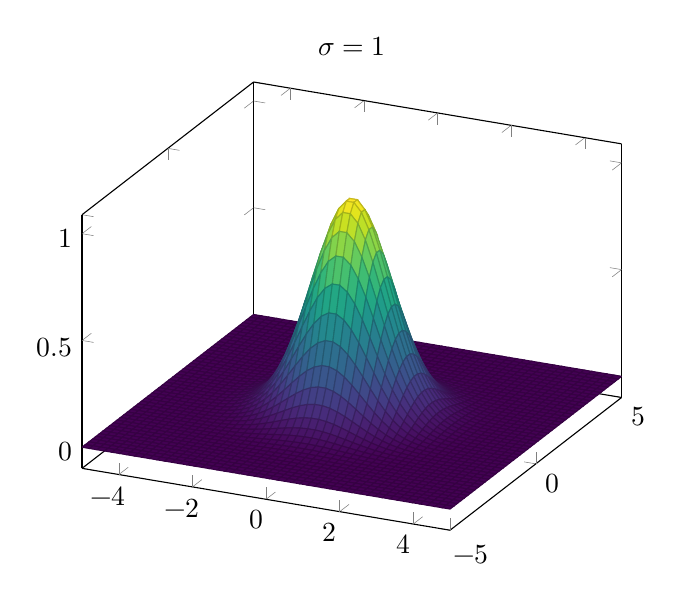
\begin{tikzpicture}
    \begin{axis}[colormap/viridis,
      title={$\sigma = 1$}]

      \addplot3[surf, samples=50] {exp(-((x^2)/2 + (y^2)/2)};
    \end{axis}
  \end{tikzpicture}

\end{document}
